\documentclass{standalone}

\usepackage{tikz}
\usetikzlibrary{arrows}
\usetikzlibrary{decorations.markings}
\usetikzlibrary{calc}
\usetikzlibrary{shapes.geometric}
\usepackage{standalone}

\begin{document}

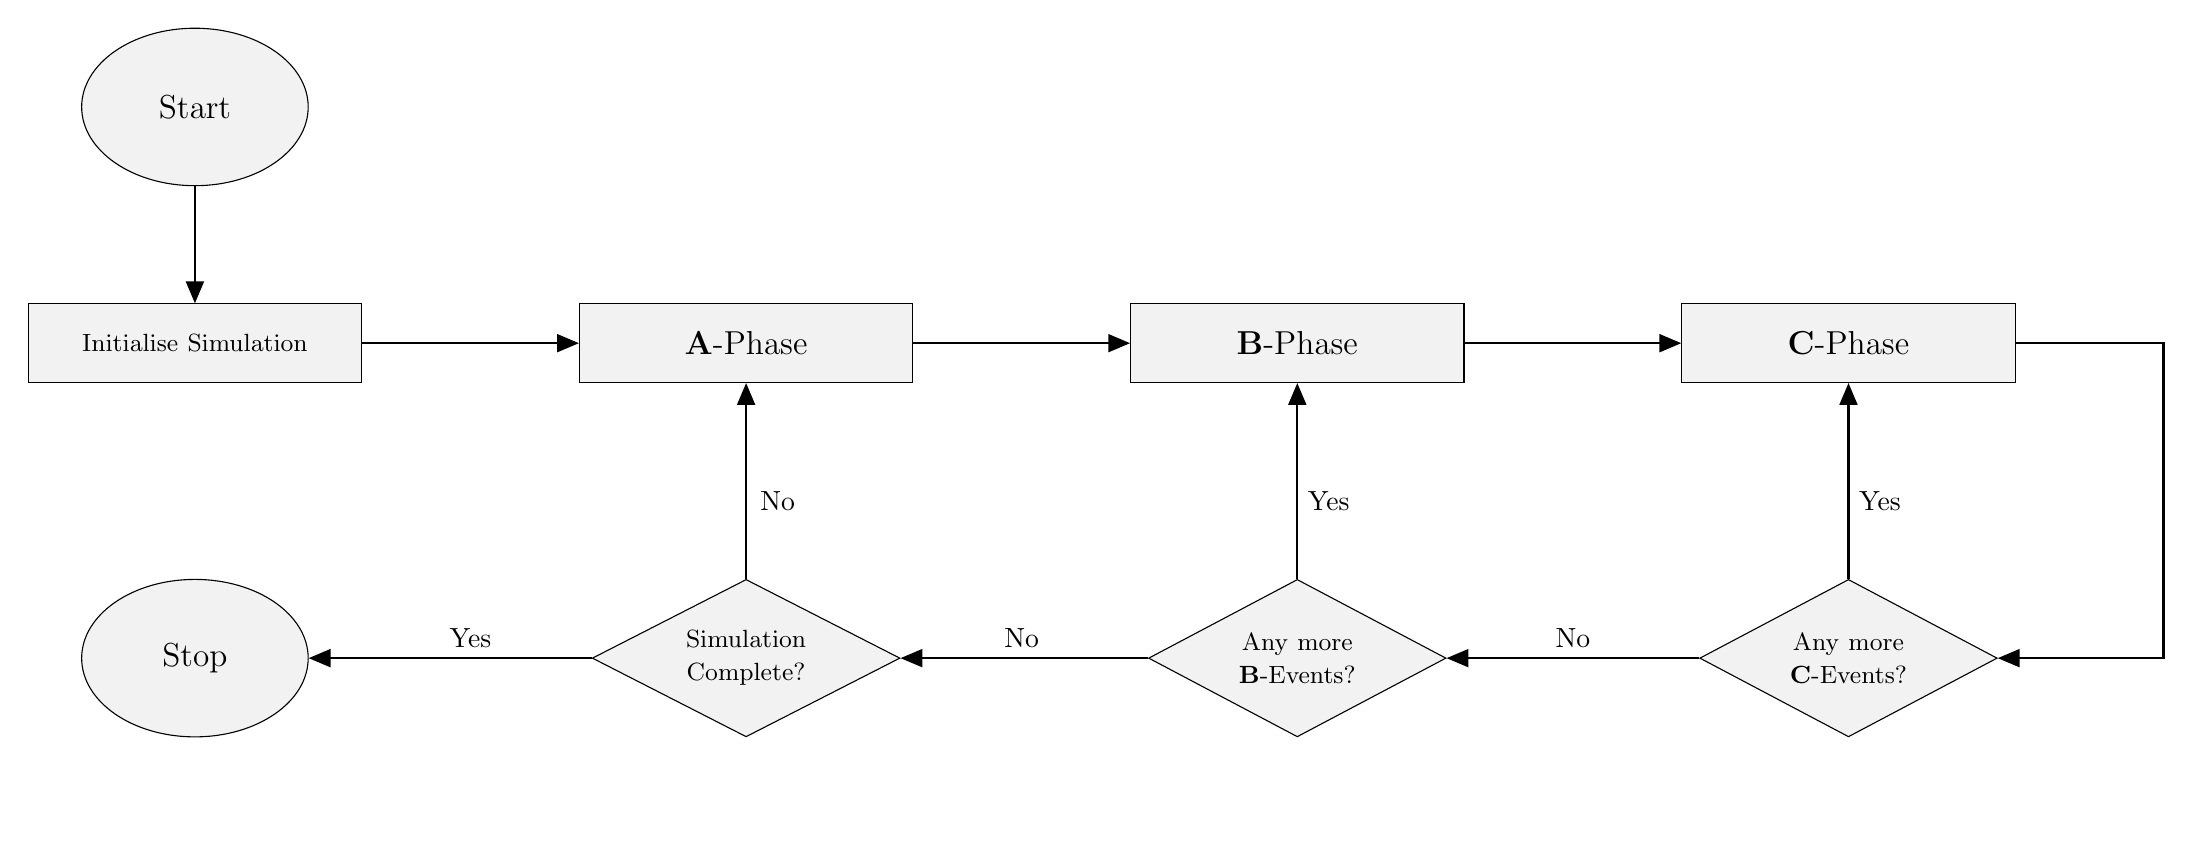
\begin{tikzpicture}

\node[align=center] (start) [style={minimum size=2cm, text width=1.8cm, draw=black,fill=black!5,text=black,shape=ellipse}] at (0, 7) {\large{Start}};


\node[align=center] (initial) [style={minimum width=3.5cm, minimum height=1cm, text width=4cm, draw=black,fill=black!5,text=black,shape=rectangle}] at (0, 4) {\small{Initialise Simulation}};

\node[align=center] (Aphase) [style={minimum width=3.5cm, minimum height=1cm, text width=4cm, draw=black,fill=black!5,text=black,shape=rectangle}] at (7, 4) {\large{\textbf{A}-Phase}};
\node[align=center] (Bphase) [style={minimum width=3.5cm, minimum height=1cm, text width=4cm, draw=black,fill=black!5,text=black,shape=rectangle}] at (14, 4) {\large{\textbf{B}-Phase}};
\node[align=center] (Cphase) [style={minimum width=3.5cm, minimum height=1cm, text width=4cm, draw=black,fill=black!5,text=black,shape=rectangle}] at (21, 4) {\large{\textbf{C}-Phase}};

\node[align=center] (anymoreC) [style={minimum size=2cm, text width=1.8cm, draw=black,fill=black!5,text=black,shape=diamond, aspect=2}] at (21, 0) {\small{Any more \textbf{C}-Events?}};
\node[align=center] (anymoreB) [style={minimum size=2cm, text width=1.8cm, draw=black,fill=black!5,text=black,shape=diamond, aspect=2}] at (14, 0) {\small{Any more \textbf{B}-Events?}};
\node[align=center] (isend) [style={minimum size=2cm, text width=1.8cm, draw=black,fill=black!5,text=black,shape=diamond, aspect=2}] at (7, 0) {\small{Simulation Complete?}};

\node[align=center] (stop) [style={minimum size=2cm, text width=1.8cm, draw=black,fill=black!5,text=black,shape=ellipse}] at (0, 0) {\large{Stop}};

\draw[draw=none] (0, 0) -- (0, -2);

\draw[thick, -triangle 45] (start) -- (initial);
\draw[thick, -triangle 45] (initial) -- (Aphase);
\draw[thick, -triangle 45] (Aphase) -- (Bphase);
\draw[thick, -triangle 45] (Bphase) -- (Cphase);
\draw[thick, -triangle 45] (anymoreC) -- (Cphase);
\draw[thick, -triangle 45] (anymoreC) -- (anymoreB);
\draw[thick, -triangle 45] (anymoreB) -- (isend);
\draw[thick, -triangle 45] (isend) -- (stop);
\draw[thick, -triangle 45] (Cphase) -- (25, 4) -- (25, 0) -- (anymoreC);
\draw[thick, -triangle 45] (anymoreB) -- (Bphase);
\draw[thick, -triangle 45] (isend) -- (Aphase);

\node at (3.5, 0.25) {Yes};
\node at (10.5, 0.25) {No};
\node at (17.5, 0.25) {No};
\node at (7.4, 2) {No};
\node at (14.4, 2) {Yes};
\node at (21.4, 2) {Yes};



\end{tikzpicture}

\end{document}
